\subsection{Coverage and computational outcomes}
The 13 registered cases are a designed product suite, not a random sample from operating mines. Figure~\ref{fig:case-inventory} counts the declared case categories and therefore describes coverage of the benchmark suite only; it cannot estimate the prevalence of any geology or operating condition. Figure~\ref{fig:method-case-coverage} reports whether a method row is present in each trace. A missing cell means that the trace contains no result row, not that the method returned a value of zero. Figure~\ref{fig:method-row-counts} makes this distinction visible at the case level. Method gaps in Figure~\ref{fig:method-gap-distribution} are taken from each row's own certified-bound comparison; the distributions must not be ranked across different mathematical formulations as though all methods shared one feasible region.

\begin{figure}[htbp]\centering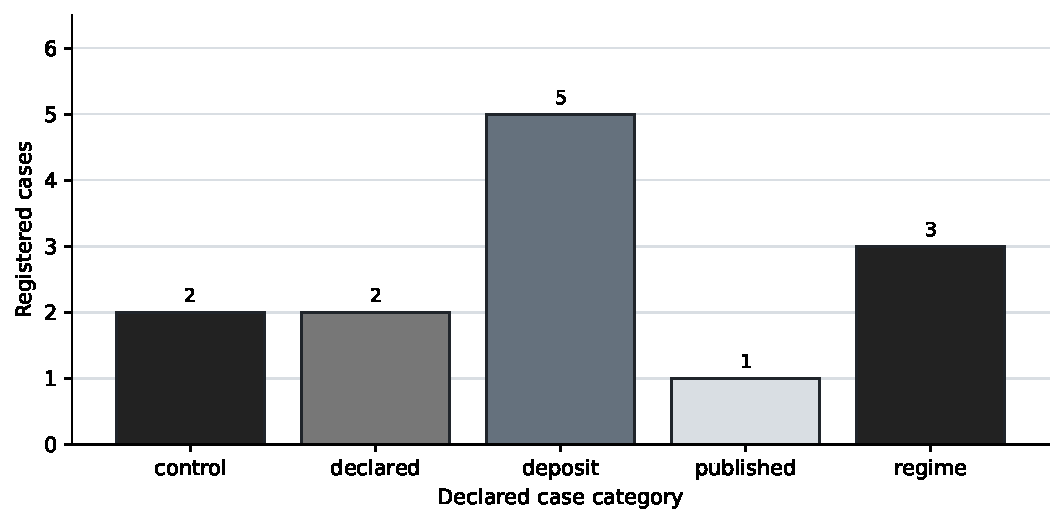
\includegraphics[width=0.82\textwidth]{figures/case-inventory.pdf}\caption{Counts of registered PhaseFlow cases by declared category, derived from the versioned manifest index and limited to this benchmark suite.}\label{fig:case-inventory}\end{figure}
\begin{figure}[htbp]\centering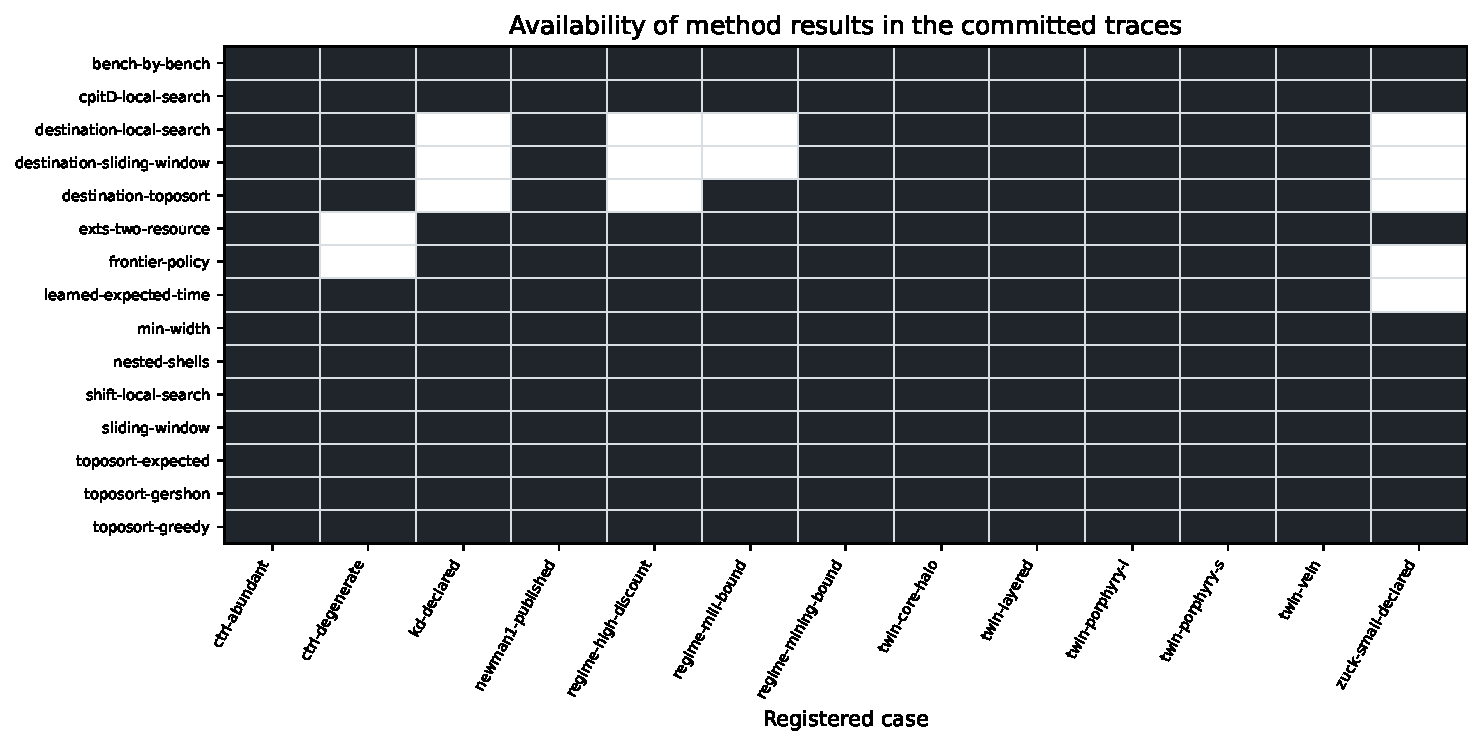
\includegraphics[width=\textwidth]{figures/method-case-coverage.pdf}\caption{Presence of a method result row in each of the thirteen committed traces; a blank cell denotes absent evidence rather than a zero-valued schedule.}\label{fig:method-case-coverage}\end{figure}
\begin{figure}[htbp]\centering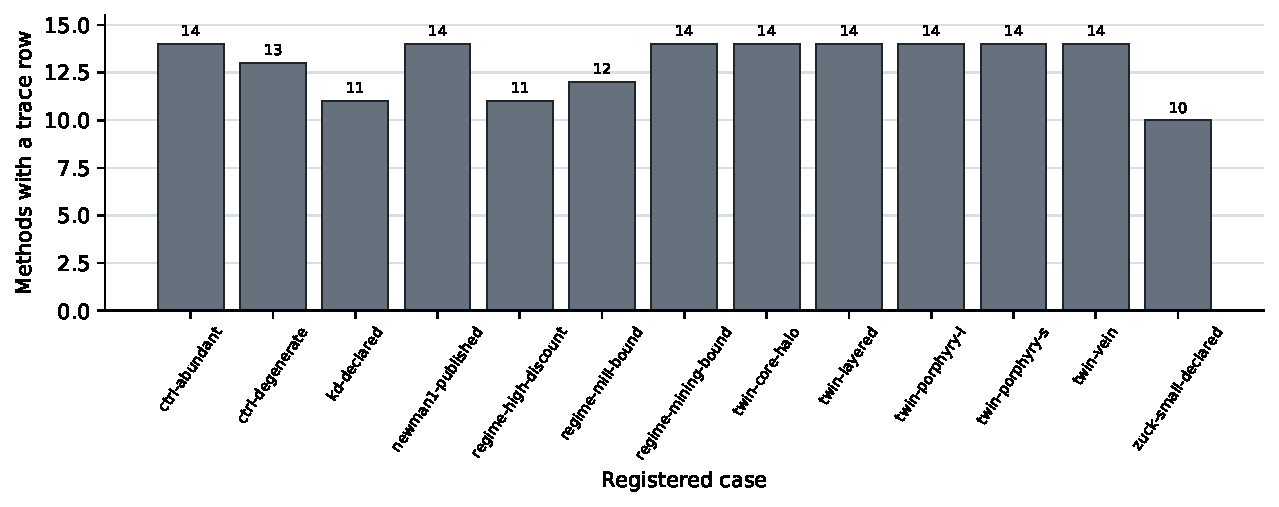
\includegraphics[width=0.9\textwidth]{figures/method-row-counts.pdf}\caption{Number of method rows in every registered case trace, showing where comparisons have different coverage and must not be treated as balanced panels.}\label{fig:method-row-counts}\end{figure}
\begin{figure}[htbp]\centering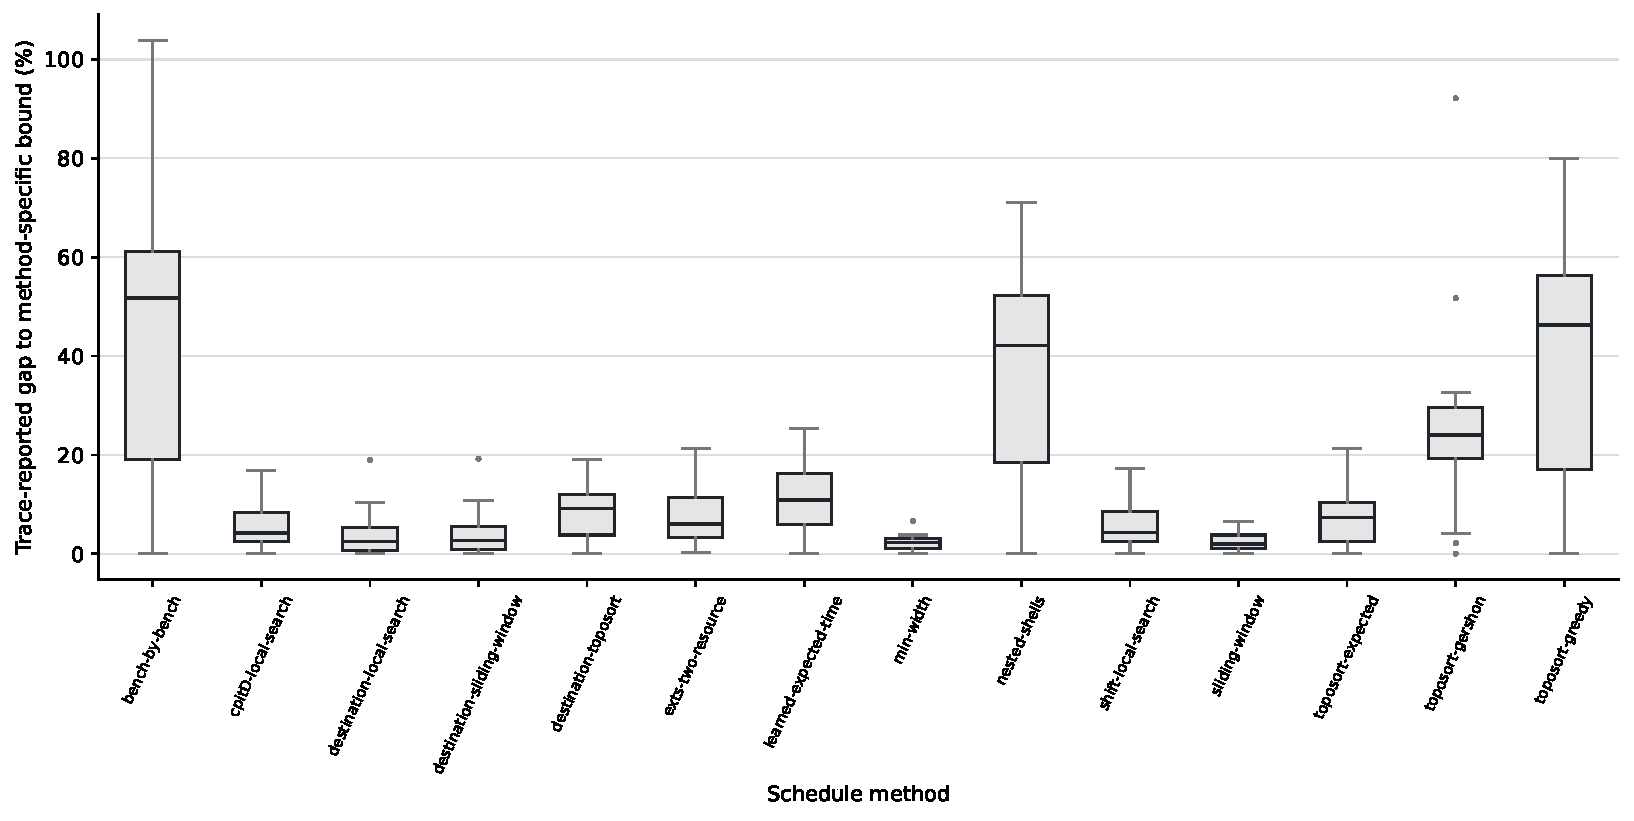
\includegraphics[width=\textwidth]{figures/method-gap-distribution.pdf}\caption{Trace-reported percentage gaps for each method against its own applicable bound across available cases; the plot does not equate distinct formulations.}\label{fig:method-gap-distribution}\end{figure}
\clearpage

The runtime comparison in Figure~\ref{fig:method-runtime} uses wall-clock milliseconds recorded by the pipeline and a logarithmic vertical scale. It shows orders-of-magnitude differences between constructive passes and restricted optimization, but the 13 product cases do not establish asymptotic complexity. Figure~\ref{fig:bound-route-difference} compares the joint and Algorithm 4 bounds only where both are computed. Differences close to zero reflect agreement within the documented column-generation tolerance for those cases; they do not prove that the two routines agree on every CPIT instance. The capacity utilization profile in Figure~\ref{fig:capacity-profile} is from the loose-capacity control and shows period-level use, not a utilization estimate for a mine plan.

Table~\ref{tab:case-method-outcomes} gives the complete case-by-method record from the committed 0.11 benchmark traces. NPV and bound retain each case's source units and should be compared within a case; the gap is the trace-reported percentage and runtime is in milliseconds. Each fixed case-method execution contributes one recorded outcome; repeated runs and inferential uncertainty estimates are unavailable, so the table reports observations rather than confidence intervals. A “no row” entry means the trace emitted no result for that pair and does not mean zero value, infeasibility, or a failed run.

\begingroup\scriptsize\setlength{\tabcolsep}{2.4pt}
\begin{longtable}{>{\raggedright\arraybackslash}p{0.16\textwidth}>{\raggedright\arraybackslash}p{0.25\textwidth}r r r r r}
\caption{Complete recorded outcomes for every registered case and every method observed in the committed 0.11 benchmark traces; missing method rows are shown explicitly and are not imputed.}\label{tab:case-method-outcomes}\\
\toprule Case & Method & Status & \shortstack{NPV\\(case units)} & \shortstack{Bound\\(case units)} & Gap (\%) & Runtime (ms) \\ \midrule\endfirsthead
\toprule Case & Method & Status & \shortstack{NPV\\(case units)} & \shortstack{Bound\\(case units)} & Gap (\%) & Runtime (ms) \\ \midrule\endhead
\texttt{ctrl\allowbreak-abundant} & \texttt{bench\allowbreak-by\allowbreak-bench} & recorded & 398634009.81 & 428750526.53 & 7.0243 & 66.6 \\
\texttt{ctrl\allowbreak-abundant} & \texttt{cpitD\allowbreak-local\allowbreak-search} & recorded & 427644502.81 & 428750526.53 & 0.2580 & 706.0 \\
\texttt{ctrl\allowbreak-abundant} & \texttt{destination\allowbreak-local\allowbreak-search} & recorded & 438028476.84 & 438824758.78 & 0.1815 & 5319.0 \\
\texttt{ctrl\allowbreak-abundant} & \texttt{destination\allowbreak-sliding\allowbreak-window} & recorded & 437899435.07 & 438824758.78 & 0.2109 & 637064.6 \\
\texttt{ctrl\allowbreak-abundant} & \texttt{destination\allowbreak-toposort} & recorded & 437075857.86 & 438824758.78 & 0.3985 & 10335.7 \\
\texttt{ctrl\allowbreak-abundant} & \texttt{exts\allowbreak-two\allowbreak-resource} & recorded & 427325801.23 & 428750526.53 & 0.3323 & 12433.5 \\
\texttt{ctrl\allowbreak-abundant} & \texttt{frontier\allowbreak-policy} & recorded & 413153254.41 & 428750526.53 & 3.6378 & 225500.0 \\
\texttt{ctrl\allowbreak-abundant} & \texttt{learned\allowbreak-expected\allowbreak-time} & recorded & 423393914.47 & 428750526.53 & 1.2494 & 1416.6 \\
\texttt{ctrl\allowbreak-abundant} & \texttt{min\allowbreak-width} & recorded & 427631215.80 & 428750526.53 & 0.2611 & 349.5 \\
\texttt{ctrl\allowbreak-abundant} & \texttt{nested\allowbreak-shells} & recorded & 404889615.93 & 428750526.53 & 5.5652 & 70.3 \\
\texttt{ctrl\allowbreak-abundant} & \texttt{shift\allowbreak-local\allowbreak-search} & recorded & 427637345.93 & 428750526.53 & 0.2596 & 60.1 \\
\texttt{ctrl\allowbreak-abundant} & \texttt{sliding\allowbreak-window} & recorded & 425960870.97 & 428750526.53 & 0.6506 & 234949.2 \\
\texttt{ctrl\allowbreak-abundant} & \texttt{toposort\allowbreak-expected} & recorded & 427325801.23 & 428750526.53 & 0.3323 & 12363.0 \\
\texttt{ctrl\allowbreak-abundant} & \texttt{toposort\allowbreak-gershon} & recorded & 419591568.06 & 428750526.53 & 2.1362 & 195.7 \\
\texttt{ctrl\allowbreak-abundant} & \texttt{toposort\allowbreak-greedy} & recorded & 401470358.50 & 428750526.53 & 6.3627 & 61.7 \\
\texttt{ctrl\allowbreak-degenerate} & \texttt{bench\allowbreak-by\allowbreak-bench} & recorded & 473615065.85 & 473615065.85 & 0.0000 & 87.7 \\
\texttt{ctrl\allowbreak-degenerate} & \texttt{cpitD\allowbreak-local\allowbreak-search} & recorded & 473615065.85 & 473615065.85 & 0.0000 & 338.8 \\
\texttt{ctrl\allowbreak-degenerate} & \texttt{destination\allowbreak-local\allowbreak-search} & recorded & 473615065.85 & 473615065.85 & 0.0000 & 779.6 \\
\texttt{ctrl\allowbreak-degenerate} & \texttt{destination\allowbreak-sliding\allowbreak-window} & recorded & 473615065.85 & 473615065.85 & 0.0000 & 3451.0 \\
\texttt{ctrl\allowbreak-degenerate} & \texttt{destination\allowbreak-toposort} & recorded & 473615065.85 & 473615065.85 & 0.0000 & 523.8 \\
\texttt{ctrl\allowbreak-degenerate} & \texttt{exts\allowbreak-two\allowbreak-resource} & no row & -- & -- & -- & -- \\
\texttt{ctrl\allowbreak-degenerate} & \texttt{frontier\allowbreak-policy} & no row & -- & -- & -- & -- \\
\texttt{ctrl\allowbreak-degenerate} & \texttt{learned\allowbreak-expected\allowbreak-time} & recorded & 473615065.85 & 473615065.85 & 0.0000 & 262.5 \\
\texttt{ctrl\allowbreak-degenerate} & \texttt{min\allowbreak-width} & recorded & 473615065.85 & 473615065.85 & 0.0000 & 334.7 \\
\texttt{ctrl\allowbreak-degenerate} & \texttt{nested\allowbreak-shells} & recorded & 473615065.85 & 473615065.85 & 0.0000 & 78.8 \\
\texttt{ctrl\allowbreak-degenerate} & \texttt{shift\allowbreak-local\allowbreak-search} & recorded & 473615065.85 & 473615065.85 & 0.0000 & 36.3 \\
\texttt{ctrl\allowbreak-degenerate} & \texttt{sliding\allowbreak-window} & recorded & 473615065.85 & 473615065.85 & 0.0000 & 3190.6 \\
\texttt{ctrl\allowbreak-degenerate} & \texttt{toposort\allowbreak-expected} & recorded & 473615065.85 & 473615065.85 & 0.0000 & 393.8 \\
\texttt{ctrl\allowbreak-degenerate} & \texttt{toposort\allowbreak-gershon} & recorded & 473615065.85 & 473615065.85 & 0.0000 & 386.1 \\
\texttt{ctrl\allowbreak-degenerate} & \texttt{toposort\allowbreak-greedy} & recorded & 473615065.85 & 473615065.85 & 0.0000 & 104.5 \\
\texttt{kd\allowbreak-declared} & \texttt{bench\allowbreak-by\allowbreak-bench} & recorded & 161242753.99 & 254345710.51 & 36.6049 & 548.8 \\
\texttt{kd\allowbreak-declared} & \texttt{cpitD\allowbreak-local\allowbreak-search} & recorded & 216143500.33 & 254345710.51 & 15.0198 & 729.9 \\
\texttt{kd\allowbreak-declared} & \texttt{destination\allowbreak-local\allowbreak-search} & no row & -- & -- & -- & -- \\
\texttt{kd\allowbreak-declared} & \texttt{destination\allowbreak-sliding\allowbreak-window} & no row & -- & -- & -- & -- \\
\texttt{kd\allowbreak-declared} & \texttt{destination\allowbreak-toposort} & no row & -- & -- & -- & -- \\
\texttt{kd\allowbreak-declared} & \texttt{exts\allowbreak-two\allowbreak-resource} & recorded & 211382547.37 & 254345710.51 & 16.8916 & 1230282.2 \\
\texttt{kd\allowbreak-declared} & \texttt{frontier\allowbreak-policy} & recorded & 204147475.00 & 254345710.51 & 19.7362 & 747140.0 \\
\texttt{kd\allowbreak-declared} & \texttt{learned\allowbreak-expected\allowbreak-time} & recorded & 189960770.51 & 254345710.51 & 25.3139 & 1003.6 \\
\texttt{kd\allowbreak-declared} & \texttt{min\allowbreak-width} & recorded & 237448230.74 & 254345710.51 & 6.6435 & 377.5 \\
\texttt{kd\allowbreak-declared} & \texttt{nested\allowbreak-shells} & recorded & 162475932.35 & 254345710.51 & 36.1200 & 563.9 \\
\texttt{kd\allowbreak-declared} & \texttt{shift\allowbreak-local\allowbreak-search} & recorded & 215466061.97 & 254345710.51 & 15.2861 & 712.4 \\
\texttt{kd\allowbreak-declared} & \texttt{sliding\allowbreak-window} & recorded & 237922439.65 & 254345710.51 & 6.4571 & 43052723.0 \\
\texttt{kd\allowbreak-declared} & \texttt{toposort\allowbreak-expected} & recorded & 211382547.37 & 254345710.51 & 16.8916 & 1229695.9 \\
\texttt{kd\allowbreak-declared} & \texttt{toposort\allowbreak-gershon} & recorded & 122846659.80 & 254345710.51 & 51.7009 & 1781.6 \\
\texttt{kd\allowbreak-declared} & \texttt{toposort\allowbreak-greedy} & recorded & 173166103.26 & 254345710.51 & 31.9170 & 546.3 \\
\texttt{newman1\allowbreak-published} & \texttt{bench\allowbreak-by\allowbreak-bench} & recorded & 22915556.73 & 24486184.09 & 6.4143 & 10.0 \\
\texttt{newman1\allowbreak-published} & \texttt{cpitD\allowbreak-local\allowbreak-search} & recorded & 23875537.97 & 24486184.09 & 2.4938 & 5370.1 \\
\texttt{newman1\allowbreak-published} & \texttt{destination\allowbreak-local\allowbreak-search} & recorded & 23875640.91 & 24486549.02 & 2.4949 & 16947.4 \\
\texttt{newman1\allowbreak-published} & \texttt{destination\allowbreak-sliding\allowbreak-window} & recorded & 23428618.76 & 24486549.02 & 4.3205 & 19304.9 \\
\texttt{newman1\allowbreak-published} & \texttt{destination\allowbreak-toposort} & recorded & 23864348.55 & 24486549.02 & 2.5410 & 1530.6 \\
\texttt{newman1\allowbreak-published} & \texttt{exts\allowbreak-two\allowbreak-resource} & recorded & 23864348.55 & 24486184.09 & 2.5395 & 2400.7 \\
\texttt{newman1\allowbreak-published} & \texttt{frontier\allowbreak-policy} & recorded & 23054389.44 & 24486184.09 & 5.8474 & 9344.0 \\
\texttt{newman1\allowbreak-published} & \texttt{learned\allowbreak-expected\allowbreak-time} & recorded & 23838465.66 & 24486184.09 & 2.6452 & 42.0 \\
\texttt{newman1\allowbreak-published} & \texttt{min\allowbreak-width} & recorded & 23872009.30 & 24486184.09 & 2.5083 & 54.0 \\
\texttt{newman1\allowbreak-published} & \texttt{nested\allowbreak-shells} & recorded & 23839631.29 & 24486184.09 & 2.6405 & 9.6 \\
\texttt{newman1\allowbreak-published} & \texttt{shift\allowbreak-local\allowbreak-search} & recorded & 23873589.42 & 24486184.09 & 2.5018 & 10.7 \\
\texttt{newman1\allowbreak-published} & \texttt{sliding\allowbreak-window} & recorded & 23428618.76 & 24486184.09 & 4.3190 & 44610.0 \\
\texttt{newman1\allowbreak-published} & \texttt{toposort\allowbreak-expected} & recorded & 23864348.55 & 24486184.09 & 2.5395 & 2390.7 \\
\texttt{newman1\allowbreak-published} & \texttt{toposort\allowbreak-gershon} & recorded & 23474084.43 & 24486184.09 & 4.1333 & 25.1 \\
\texttt{newman1\allowbreak-published} & \texttt{toposort\allowbreak-greedy} & recorded & 23552841.72 & 24486184.09 & 3.8117 & 15.0 \\
\texttt{regime\allowbreak-high\allowbreak-discount} & \texttt{bench\allowbreak-by\allowbreak-bench} & recorded & 71675727.37 & 184634636.79 & 61.1797 & 62.6 \\
\texttt{regime\allowbreak-high\allowbreak-discount} & \texttt{cpitD\allowbreak-local\allowbreak-search} & recorded & 169795008.10 & 184634636.79 & 8.0373 & 970.4 \\
\texttt{regime\allowbreak-high\allowbreak-discount} & \texttt{destination\allowbreak-local\allowbreak-search} & no row & -- & -- & -- & -- \\
\texttt{regime\allowbreak-high\allowbreak-discount} & \texttt{destination\allowbreak-sliding\allowbreak-window} & no row & -- & -- & -- & -- \\
\texttt{regime\allowbreak-high\allowbreak-discount} & \texttt{destination\allowbreak-toposort} & no row & -- & -- & -- & -- \\
\texttt{regime\allowbreak-high\allowbreak-discount} & \texttt{exts\allowbreak-two\allowbreak-resource} & recorded & 168506774.83 & 184634636.79 & 8.7350 & 18649.2 \\
\texttt{regime\allowbreak-high\allowbreak-discount} & \texttt{frontier\allowbreak-policy} & recorded & 159223871.11 & 184634636.79 & 13.7627 & 63328.0 \\
\texttt{regime\allowbreak-high\allowbreak-discount} & \texttt{learned\allowbreak-expected\allowbreak-time} & recorded & 167477586.97 & 184634636.79 & 9.2924 & 10405.9 \\
\texttt{regime\allowbreak-high\allowbreak-discount} & \texttt{min\allowbreak-width} & recorded & 181077135.78 & 184634636.79 & 1.9268 & 1172.4 \\
\texttt{regime\allowbreak-high\allowbreak-discount} & \texttt{nested\allowbreak-shells} & recorded & 88065737.46 & 184634636.79 & 52.3027 & 60.9 \\
\texttt{regime\allowbreak-high\allowbreak-discount} & \texttt{shift\allowbreak-local\allowbreak-search} & recorded & 169738335.86 & 184634636.79 & 8.0680 & 43.1 \\
\texttt{regime\allowbreak-high\allowbreak-discount} & \texttt{sliding\allowbreak-window} & recorded & 181093517.32 & 184634636.79 & 1.9179 & 870157.4 \\
\texttt{regime\allowbreak-high\allowbreak-discount} & \texttt{toposort\allowbreak-expected} & recorded & 168506774.83 & 184634636.79 & 8.7350 & 18586.7 \\
\texttt{regime\allowbreak-high\allowbreak-discount} & \texttt{toposort\allowbreak-gershon} & recorded & 141804901.67 & 184634636.79 & 23.1970 & 182.1 \\
\texttt{regime\allowbreak-high\allowbreak-discount} & \texttt{toposort\allowbreak-greedy} & recorded & 80712545.33 & 184634636.79 & 56.2853 & 61.1 \\
\texttt{regime\allowbreak-mill\allowbreak-bound} & \texttt{bench\allowbreak-by\allowbreak-bench} & recorded & 27438402.44 & 129686447.19 & 78.8425 & 112.1 \\
\texttt{regime\allowbreak-mill\allowbreak-bound} & \texttt{cpitD\allowbreak-local\allowbreak-search} & recorded & 112011241.62 & 129686447.19 & 13.6292 & 3957.9 \\
\texttt{regime\allowbreak-mill\allowbreak-bound} & \texttt{destination\allowbreak-local\allowbreak-search} & no row & -- & -- & -- & -- \\
\texttt{regime\allowbreak-mill\allowbreak-bound} & \texttt{destination\allowbreak-sliding\allowbreak-window} & no row & -- & -- & -- & -- \\
\texttt{regime\allowbreak-mill\allowbreak-bound} & \texttt{destination\allowbreak-toposort} & recorded & 190273768.14 & 207638996.94 & 8.3632 & 76867.0 \\
\texttt{regime\allowbreak-mill\allowbreak-bound} & \texttt{exts\allowbreak-two\allowbreak-resource} & recorded & 110317470.62 & 129686447.19 & 14.9352 & 37493.1 \\
\texttt{regime\allowbreak-mill\allowbreak-bound} & \texttt{frontier\allowbreak-policy} & recorded & 101124141.73 & 129686447.19 & 22.0241 & 41891.0 \\
\texttt{regime\allowbreak-mill\allowbreak-bound} & \texttt{learned\allowbreak-expected\allowbreak-time} & recorded & 112281367.00 & 129686447.19 & 13.4209 & 339.1 \\
\texttt{regime\allowbreak-mill\allowbreak-bound} & \texttt{min\allowbreak-width} & recorded & 124764860.94 & 129686447.19 & 3.7950 & 117.8 \\
\texttt{regime\allowbreak-mill\allowbreak-bound} & \texttt{nested\allowbreak-shells} & recorded & 37413390.52 & 129686447.19 & 71.1509 & 107.9 \\
\texttt{regime\allowbreak-mill\allowbreak-bound} & \texttt{shift\allowbreak-local\allowbreak-search} & recorded & 111801028.46 & 129686447.19 & 13.7913 & 68.3 \\
\texttt{regime\allowbreak-mill\allowbreak-bound} & \texttt{sliding\allowbreak-window} & recorded & 124764198.75 & 129686447.19 & 3.7955 & 8094593.2 \\
\texttt{regime\allowbreak-mill\allowbreak-bound} & \texttt{toposort\allowbreak-expected} & recorded & 110317470.62 & 129686447.19 & 14.9352 & 37373.2 \\
\texttt{regime\allowbreak-mill\allowbreak-bound} & \texttt{toposort\allowbreak-gershon} & recorded & 91229398.23 & 129686447.19 & 29.6539 & 423.3 \\
\texttt{regime\allowbreak-mill\allowbreak-bound} & \texttt{toposort\allowbreak-greedy} & recorded & 37580828.14 & 129686447.19 & 71.0218 & 97.1 \\
\texttt{regime\allowbreak-mining\allowbreak-bound} & \texttt{bench\allowbreak-by\allowbreak-bench} & recorded & 46282695.39 & 187991036.34 & 75.3804 & 97.8 \\
\texttt{regime\allowbreak-mining\allowbreak-bound} & \texttt{cpitD\allowbreak-local\allowbreak-search} & recorded & 173959432.24 & 187991036.34 & 7.4640 & 1354.4 \\
\texttt{regime\allowbreak-mining\allowbreak-bound} & \texttt{destination\allowbreak-local\allowbreak-search} & recorded & 182965952.37 & 187991036.34 & 2.6730 & 2547.9 \\
\texttt{regime\allowbreak-mining\allowbreak-bound} & \texttt{destination\allowbreak-sliding\allowbreak-window} & recorded & 182955948.65 & 187991036.34 & 2.6784 & 293727.3 \\
\texttt{regime\allowbreak-mining\allowbreak-bound} & \texttt{destination\allowbreak-toposort} & recorded & 173833944.80 & 187991036.34 & 7.5307 & 33821.0 \\
\texttt{regime\allowbreak-mining\allowbreak-bound} & \texttt{exts\allowbreak-two\allowbreak-resource} & recorded & 173936547.76 & 187991036.34 & 7.4761 & 27157.4 \\
\texttt{regime\allowbreak-mining\allowbreak-bound} & \texttt{frontier\allowbreak-policy} & recorded & 136789708.76 & 187991036.34 & 27.2360 & 52953.0 \\
\texttt{regime\allowbreak-mining\allowbreak-bound} & \texttt{learned\allowbreak-expected\allowbreak-time} & recorded & 165775509.75 & 187991036.34 & 11.8173 & 250.9 \\
\texttt{regime\allowbreak-mining\allowbreak-bound} & \texttt{min\allowbreak-width} & recorded & 182955948.65 & 187991036.34 & 2.6784 & 104.5 \\
\texttt{regime\allowbreak-mining\allowbreak-bound} & \texttt{nested\allowbreak-shells} & recorded & 84693368.98 & 187991036.34 & 54.9482 & 91.6 \\
\texttt{regime\allowbreak-mining\allowbreak-bound} & \texttt{shift\allowbreak-local\allowbreak-search} & recorded & 173936547.76 & 187991036.34 & 7.4761 & 48.7 \\
\texttt{regime\allowbreak-mining\allowbreak-bound} & \texttt{sliding\allowbreak-window} & recorded & 182955948.65 & 187991036.34 & 2.6784 & 414483.6 \\
\texttt{regime\allowbreak-mining\allowbreak-bound} & \texttt{toposort\allowbreak-expected} & recorded & 173833944.80 & 187991036.34 & 7.5307 & 27070.9 \\
\texttt{regime\allowbreak-mining\allowbreak-bound} & \texttt{toposort\allowbreak-gershon} & recorded & 135904818.17 & 187991036.34 & 27.7068 & 344.4 \\
\texttt{regime\allowbreak-mining\allowbreak-bound} & \texttt{toposort\allowbreak-greedy} & recorded & 80886097.28 & 187991036.34 & 56.9734 & 85.4 \\
\texttt{twin\allowbreak-core\allowbreak-halo} & \texttt{bench\allowbreak-by\allowbreak-bench} & recorded & -3749944.12 & 97374025.65 & 103.8511 & 119.9 \\
\texttt{twin\allowbreak-core\allowbreak-halo} & \texttt{cpitD\allowbreak-local\allowbreak-search} & recorded & 89185799.33 & 97374025.65 & 8.4090 & 375.4 \\
\texttt{twin\allowbreak-core\allowbreak-halo} & \texttt{destination\allowbreak-local\allowbreak-search} & recorded & 124888369.55 & 131860391.69 & 5.2874 & 2017.0 \\
\texttt{twin\allowbreak-core\allowbreak-halo} & \texttt{destination\allowbreak-sliding\allowbreak-window} & recorded & 124663891.68 & 131860391.69 & 5.4577 & 100898440.8 \\
\texttt{twin\allowbreak-core\allowbreak-halo} & \texttt{destination\allowbreak-toposort} & recorded & 110093184.62 & 131860391.69 & 16.5078 & 193498.5 \\
\texttt{twin\allowbreak-core\allowbreak-halo} & \texttt{exts\allowbreak-two\allowbreak-resource} & recorded & 87353942.61 & 97374025.65 & 10.2903 & 38870.5 \\
\texttt{twin\allowbreak-core\allowbreak-halo} & \texttt{frontier\allowbreak-policy} & recorded & 12960635.64 & 97374025.65 & 86.6898 & 240375.0 \\
\texttt{twin\allowbreak-core\allowbreak-halo} & \texttt{learned\allowbreak-expected\allowbreak-time} & recorded & 76238349.72 & 97374025.65 & 21.7057 & 306.0 \\
\texttt{twin\allowbreak-core\allowbreak-halo} & \texttt{min\allowbreak-width} & recorded & 94383318.02 & 97374025.65 & 3.0714 & 333.8 \\
\texttt{twin\allowbreak-core\allowbreak-halo} & \texttt{nested\allowbreak-shells} & recorded & 32082724.70 & 97374025.65 & 67.0521 & 120.2 \\
\texttt{twin\allowbreak-core\allowbreak-halo} & \texttt{shift\allowbreak-local\allowbreak-search} & recorded & 89079079.40 & 97374025.65 & 8.5186 & 80.2 \\
\texttt{twin\allowbreak-core\allowbreak-halo} & \texttt{sliding\allowbreak-window} & recorded & 94400395.06 & 97374025.65 & 3.0538 & 4427029.4 \\
\texttt{twin\allowbreak-core\allowbreak-halo} & \texttt{toposort\allowbreak-expected} & recorded & 87353942.61 & 97374025.65 & 10.2903 & 38764.5 \\
\texttt{twin\allowbreak-core\allowbreak-halo} & \texttt{toposort\allowbreak-gershon} & recorded & 72931998.92 & 97374025.65 & 25.1012 & 431.6 \\
\texttt{twin\allowbreak-core\allowbreak-halo} & \texttt{toposort\allowbreak-greedy} & recorded & 19478724.49 & 97374025.65 & 79.9960 & 111.5 \\
\texttt{twin\allowbreak-layered} & \texttt{bench\allowbreak-by\allowbreak-bench} & recorded & 899817035.61 & 1111128368.75 & 19.0177 & 278.3 \\
\texttt{twin\allowbreak-layered} & \texttt{cpitD\allowbreak-local\allowbreak-search} & recorded & 1071699060.76 & 1111128368.75 & 3.5486 & 1504.3 \\
\texttt{twin\allowbreak-layered} & \texttt{destination\allowbreak-local\allowbreak-search} & recorded & 1223250861.55 & 1365530202.41 & 10.4193 & 15999.8 \\
\texttt{twin\allowbreak-layered} & \texttt{destination\allowbreak-sliding\allowbreak-window} & recorded & 1218078182.62 & 1365530202.41 & 10.7982 & 26903036.2 \\
\texttt{twin\allowbreak-layered} & \texttt{destination\allowbreak-toposort} & recorded & 1199918922.00 & 1365530202.41 & 12.1280 & 102246.9 \\
\texttt{twin\allowbreak-layered} & \texttt{exts\allowbreak-two\allowbreak-resource} & recorded & 1071675842.38 & 1111128368.75 & 3.5507 & 142978.2 \\
\texttt{twin\allowbreak-layered} & \texttt{frontier\allowbreak-policy} & recorded & 954631473.15 & 1111128368.75 & 14.0845 & 337594.0 \\
\texttt{twin\allowbreak-layered} & \texttt{learned\allowbreak-expected\allowbreak-time} & recorded & 943692071.51 & 1111128368.75 & 15.0690 & 467.2 \\
\texttt{twin\allowbreak-layered} & \texttt{min\allowbreak-width} & recorded & 1071699060.76 & 1111128368.75 & 3.5486 & 483.0 \\
\texttt{twin\allowbreak-layered} & \texttt{nested\allowbreak-shells} & recorded & 906350214.91 & 1111128368.75 & 18.4297 & 268.5 \\
\texttt{twin\allowbreak-layered} & \texttt{shift\allowbreak-local\allowbreak-search} & recorded & 1071675842.38 & 1111128368.75 & 3.5507 & 125.8 \\
\texttt{twin\allowbreak-layered} & \texttt{sliding\allowbreak-window} & recorded & 1043154180.50 & 1111128368.75 & 6.1176 & 61319696.8 \\
\texttt{twin\allowbreak-layered} & \texttt{toposort\allowbreak-expected} & recorded & 1071675842.38 & 1111128368.75 & 3.5507 & 142672.4 \\
\texttt{twin\allowbreak-layered} & \texttt{toposort\allowbreak-gershon} & recorded & 896014135.91 & 1111128368.75 & 19.3600 & 960.3 \\
\texttt{twin\allowbreak-layered} & \texttt{toposort\allowbreak-greedy} & recorded & 922170648.98 & 1111128368.75 & 17.0059 & 266.9 \\
\texttt{twin\allowbreak-porphyry\allowbreak-l} & \texttt{bench\allowbreak-by\allowbreak-bench} & recorded & 130457207.30 & 326536184.81 & 60.0482 & 152.7 \\
\texttt{twin\allowbreak-porphyry\allowbreak-l} & \texttt{cpitD\allowbreak-local\allowbreak-search} & recorded & 314277464.74 & 326536184.81 & 3.7542 & 554.6 \\
\texttt{twin\allowbreak-porphyry\allowbreak-l} & \texttt{destination\allowbreak-local\allowbreak-search} & recorded & 435284799.50 & 442009362.99 & 1.5214 & 2520.4 \\
\texttt{twin\allowbreak-porphyry\allowbreak-l} & \texttt{destination\allowbreak-sliding\allowbreak-window} & recorded & 434585393.36 & 442009362.99 & 1.6796 & 7597200.9 \\
\texttt{twin\allowbreak-porphyry\allowbreak-l} & \texttt{destination\allowbreak-toposort} & recorded & 391770770.21 & 442009362.99 & 11.3660 & 112771.1 \\
\texttt{twin\allowbreak-porphyry\allowbreak-l} & \texttt{exts\allowbreak-two\allowbreak-resource} & recorded & 312945549.84 & 326536184.81 & 4.1621 & 93434.3 \\
\texttt{twin\allowbreak-porphyry\allowbreak-l} & \texttt{frontier\allowbreak-policy} & recorded & 277296868.19 & 326536184.81 & 15.0793 & 140468.0 \\
\texttt{twin\allowbreak-porphyry\allowbreak-l} & \texttt{learned\allowbreak-expected\allowbreak-time} & recorded & 294357112.95 & 326536184.81 & 9.8547 & 227.6 \\
\texttt{twin\allowbreak-porphyry\allowbreak-l} & \texttt{min\allowbreak-width} & recorded & 321364047.29 & 326536184.81 & 1.5839 & 399.9 \\
\texttt{twin\allowbreak-porphyry\allowbreak-l} & \texttt{nested\allowbreak-shells} & recorded & 178634640.63 & 326536184.81 & 45.2941 & 142.8 \\
\texttt{twin\allowbreak-porphyry\allowbreak-l} & \texttt{shift\allowbreak-local\allowbreak-search} & recorded & 314247297.94 & 326536184.81 & 3.7634 & 107.6 \\
\texttt{twin\allowbreak-porphyry\allowbreak-l} & \texttt{sliding\allowbreak-window} & recorded & 321380848.23 & 326536184.81 & 1.5788 & 8228931.2 \\
\texttt{twin\allowbreak-porphyry\allowbreak-l} & \texttt{toposort\allowbreak-expected} & recorded & 302668911.25 & 326536184.81 & 7.3092 & 93282.8 \\
\texttt{twin\allowbreak-porphyry\allowbreak-l} & \texttt{toposort\allowbreak-gershon} & recorded & 248020634.26 & 326536184.81 & 24.0450 & 571.2 \\
\texttt{twin\allowbreak-porphyry\allowbreak-l} & \texttt{toposort\allowbreak-greedy} & recorded & 168760440.49 & 326536184.81 & 48.3180 & 144.8 \\
\texttt{twin\allowbreak-porphyry\allowbreak-s} & \texttt{bench\allowbreak-by\allowbreak-bench} & recorded & 107531529.28 & 234230541.78 & 54.0916 & 93.2 \\
\texttt{twin\allowbreak-porphyry\allowbreak-s} & \texttt{cpitD\allowbreak-local\allowbreak-search} & recorded & 224340746.28 & 234230541.78 & 4.2222 & 966.0 \\
\texttt{twin\allowbreak-porphyry\allowbreak-s} & \texttt{destination\allowbreak-local\allowbreak-search} & recorded & 314279336.50 & 316475407.00 & 0.6939 & 1198.4 \\
\texttt{twin\allowbreak-porphyry\allowbreak-s} & \texttt{destination\allowbreak-sliding\allowbreak-window} & recorded & 314005925.57 & 316475407.00 & 0.7803 & 5247976.1 \\
\texttt{twin\allowbreak-porphyry\allowbreak-s} & \texttt{destination\allowbreak-toposort} & recorded & 285163568.34 & 316475407.00 & 9.8939 & 54428.5 \\
\texttt{twin\allowbreak-porphyry\allowbreak-s} & \texttt{exts\allowbreak-two\allowbreak-resource} & recorded & 223413684.70 & 234230541.78 & 4.6180 & 28809.3 \\
\texttt{twin\allowbreak-porphyry\allowbreak-s} & \texttt{frontier\allowbreak-policy} & recorded & 209106102.27 & 234230541.78 & 10.7264 & 66593.0 \\
\texttt{twin\allowbreak-porphyry\allowbreak-s} & \texttt{learned\allowbreak-expected\allowbreak-time} & recorded & 217707634.04 & 234230541.78 & 7.0541 & 158.8 \\
\texttt{twin\allowbreak-porphyry\allowbreak-s} & \texttt{min\allowbreak-width} & recorded & 231603547.81 & 234230541.78 & 1.1215 & 128.0 \\
\texttt{twin\allowbreak-porphyry\allowbreak-s} & \texttt{nested\allowbreak-shells} & recorded & 130810346.26 & 234230541.78 & 44.1532 & 87.4 \\
\texttt{twin\allowbreak-porphyry\allowbreak-s} & \texttt{shift\allowbreak-local\allowbreak-search} & recorded & 224241882.03 & 234230541.78 & 4.2645 & 54.3 \\
\texttt{twin\allowbreak-porphyry\allowbreak-s} & \texttt{sliding\allowbreak-window} & recorded & 231622561.26 & 234230541.78 & 1.1134 & 3166607.9 \\
\texttt{twin\allowbreak-porphyry\allowbreak-s} & \texttt{toposort\allowbreak-expected} & recorded & 223413684.70 & 234230541.78 & 4.6180 & 28726.8 \\
\texttt{twin\allowbreak-porphyry\allowbreak-s} & \texttt{toposort\allowbreak-gershon} & recorded & 187236534.51 & 234230541.78 & 20.0631 & 299.7 \\
\texttt{twin\allowbreak-porphyry\allowbreak-s} & \texttt{toposort\allowbreak-greedy} & recorded & 117596777.73 & 234230541.78 & 49.7944 & 80.9 \\
\texttt{twin\allowbreak-vein} & \texttt{bench\allowbreak-by\allowbreak-bench} & recorded & 172734791.93 & 285385073.56 & 39.4731 & 231.7 \\
\texttt{twin\allowbreak-vein} & \texttt{cpitD\allowbreak-local\allowbreak-search} & recorded & 283628430.36 & 285385073.56 & 0.6155 & 985.4 \\
\texttt{twin\allowbreak-vein} & \texttt{destination\allowbreak-local\allowbreak-search} & recorded & 300153975.44 & 370316500.73 & 18.9466 & 8967.0 \\
\texttt{twin\allowbreak-vein} & \texttt{destination\allowbreak-sliding\allowbreak-window} & recorded & 299142002.02 & 370316500.73 & 19.2199 & 3689975.7 \\
\texttt{twin\allowbreak-vein} & \texttt{destination\allowbreak-toposort} & recorded & 299979371.52 & 370316500.73 & 18.9938 & 357718.2 \\
\texttt{twin\allowbreak-vein} & \texttt{exts\allowbreak-two\allowbreak-resource} & recorded & 280993395.08 & 285385073.56 & 1.5389 & 93610.0 \\
\texttt{twin\allowbreak-vein} & \texttt{frontier\allowbreak-policy} & recorded & 223609743.51 & 285385073.56 & 21.6463 & 220563.0 \\
\texttt{twin\allowbreak-vein} & \texttt{learned\allowbreak-expected\allowbreak-time} & recorded & 229200036.05 & 285385073.56 & 19.6874 & 407.9 \\
\texttt{twin\allowbreak-vein} & \texttt{min\allowbreak-width} & recorded & 285102255.15 & 285385073.56 & 0.0991 & 690.8 \\
\texttt{twin\allowbreak-vein} & \texttt{nested\allowbreak-shells} & recorded & 165147496.81 & 285385073.56 & 42.1317 & 222.7 \\
\texttt{twin\allowbreak-vein} & \texttt{shift\allowbreak-local\allowbreak-search} & recorded & 283568073.89 & 285385073.56 & 0.6367 & 147.9 \\
\texttt{twin\allowbreak-vein} & \texttt{sliding\allowbreak-window} & recorded & 285108029.53 & 285385073.56 & 0.0971 & 2062209.0 \\
\texttt{twin\allowbreak-vein} & \texttt{toposort\allowbreak-expected} & recorded & 280993395.08 & 285385073.56 & 1.5389 & 93387.5 \\
\texttt{twin\allowbreak-vein} & \texttt{toposort\allowbreak-gershon} & recorded & 22428664.26 & 285385073.56 & 92.1409 & 1024.9 \\
\texttt{twin\allowbreak-vein} & \texttt{toposort\allowbreak-greedy} & recorded & 181068401.86 & 285385073.56 & 36.5530 & 217.9 \\
\texttt{zuck\allowbreak-small\allowbreak-declared} & \texttt{bench\allowbreak-by\allowbreak-bench} & recorded & 346832457.33 & 719234226.20 & 51.7775 & 276.7 \\
\texttt{zuck\allowbreak-small\allowbreak-declared} & \texttt{cpitD\allowbreak-local\allowbreak-search} & recorded & 597620803.33 & 719234226.20 & 16.9087 & 454.1 \\
\texttt{zuck\allowbreak-small\allowbreak-declared} & \texttt{destination\allowbreak-local\allowbreak-search} & no row & -- & -- & -- & -- \\
\texttt{zuck\allowbreak-small\allowbreak-declared} & \texttt{destination\allowbreak-sliding\allowbreak-window} & no row & -- & -- & -- & -- \\
\texttt{zuck\allowbreak-small\allowbreak-declared} & \texttt{destination\allowbreak-toposort} & no row & -- & -- & -- & -- \\
\texttt{zuck\allowbreak-small\allowbreak-declared} & \texttt{exts\allowbreak-two\allowbreak-resource} & recorded & 566520496.41 & 719234226.20 & 21.2328 & 254238.3 \\
\texttt{zuck\allowbreak-small\allowbreak-declared} & \texttt{frontier\allowbreak-policy} & no row & -- & -- & -- & -- \\
\texttt{zuck\allowbreak-small\allowbreak-declared} & \texttt{learned\allowbreak-expected\allowbreak-time} & no row & -- & -- & -- & -- \\
\texttt{zuck\allowbreak-small\allowbreak-declared} & \texttt{min\allowbreak-width} & recorded & 703210120.67 & 719234226.20 & 2.2279 & 314.5 \\
\texttt{zuck\allowbreak-small\allowbreak-declared} & \texttt{nested\allowbreak-shells} & recorded & 495393569.72 & 719234226.20 & 31.1221 & 256.9 \\
\texttt{zuck\allowbreak-small\allowbreak-declared} & \texttt{shift\allowbreak-local\allowbreak-search} & recorded & 594985768.04 & 719234226.20 & 17.2751 & 427.3 \\
\texttt{zuck\allowbreak-small\allowbreak-declared} & \texttt{sliding\allowbreak-window} & recorded & 705009489.02 & 719234226.20 & 1.9778 & 6579257.9 \\
\texttt{zuck\allowbreak-small\allowbreak-declared} & \texttt{toposort\allowbreak-expected} & recorded & 565706313.09 & 719234226.20 & 21.3460 & 253978.8 \\
\texttt{zuck\allowbreak-small\allowbreak-declared} & \texttt{toposort\allowbreak-gershon} & recorded & 483991842.71 & 719234226.20 & 32.7073 & 735.6 \\
\texttt{zuck\allowbreak-small\allowbreak-declared} & \texttt{toposort\allowbreak-greedy} & recorded & 386377893.10 & 719234226.20 & 46.2793 & 249.7 \\
\bottomrule\end{longtable}\endgroup

\clearpage

\begin{figure}[htbp]\centering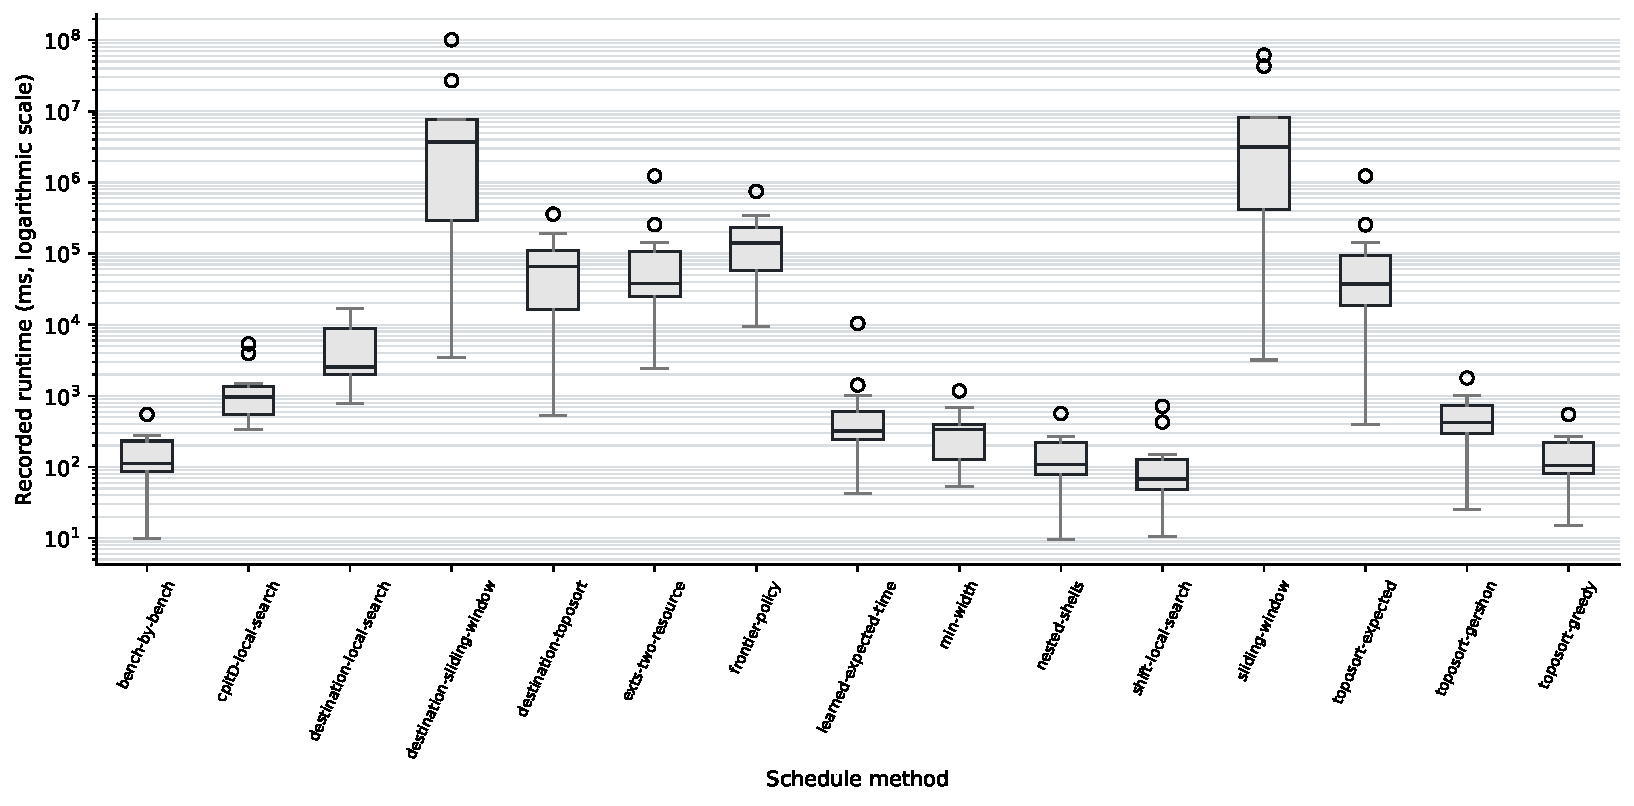
\includegraphics[width=\textwidth]{figures/method-runtime.pdf}\caption{Recorded runtime distributions by schedule method over the cases that contain a runtime, with logarithmic scaling preserving both short constructive passes and long optimization runs.}\label{fig:method-runtime}\end{figure}
\begin{figure}[htbp]\centering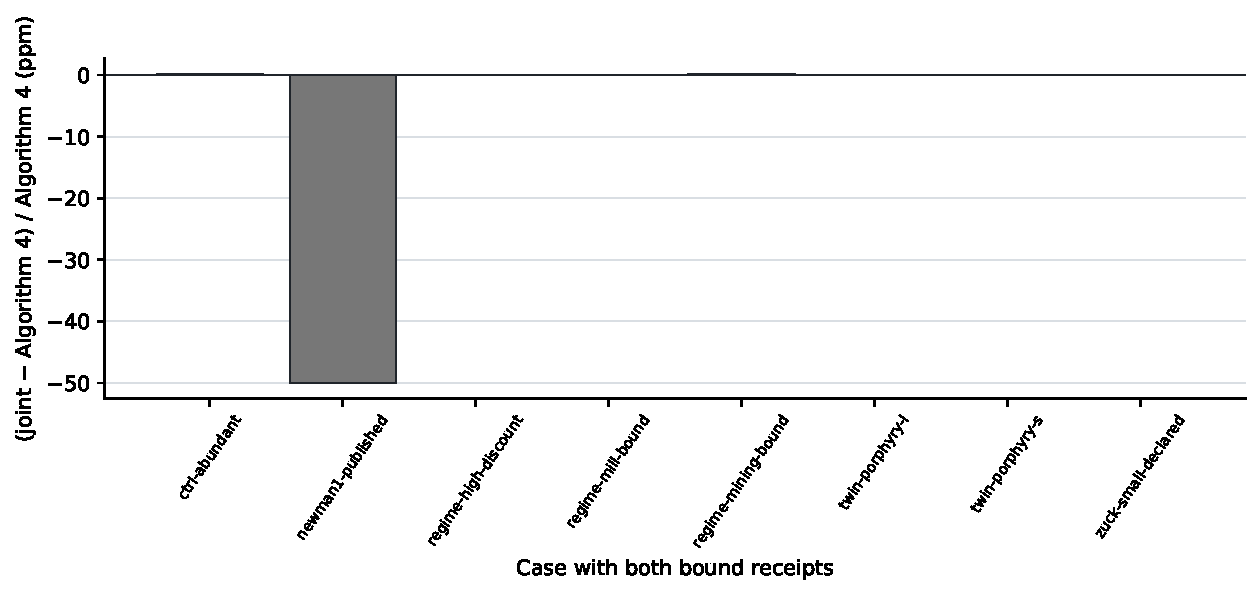
\includegraphics[width=0.82\textwidth]{figures/bound-route-difference.pdf}\caption{Relative difference in parts per million between two upper-bound computations on cases where both are present, retaining the sign and the bound provenance.}\label{fig:bound-route-difference}\end{figure}
\begin{figure}[htbp]\centering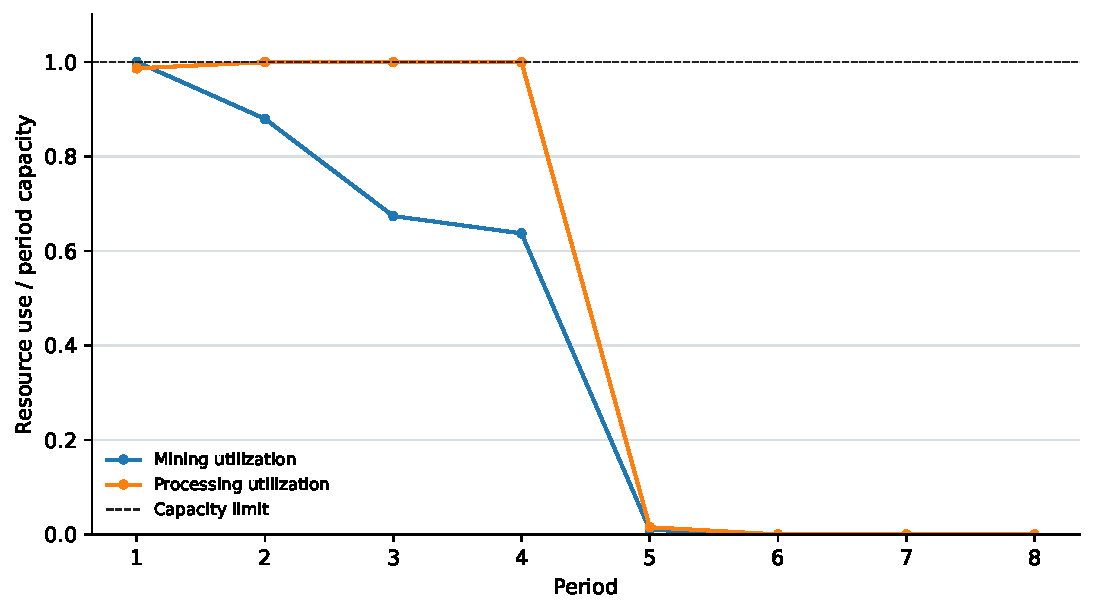
\includegraphics[width=0.82\textwidth]{figures/capacity-profile.pdf}\caption{Period resource utilization for the declared loose-capacity diagnostic, calculated from the selected trace's mined tonnes and resource limits.}\label{fig:capacity-profile}\end{figure}
\clearpage

Table~\ref{tab:method-result-summary} is the trace-level detail behind the method coverage and runtime summaries: the
available row count ranges from 9 to 13 cases, and the destination sliding-window trace reaches 100,898,440.8 ms,
compared with 548.8 ms for the bench-by-bench constructor. These are observed runtimes on this fixed suite, not
complexity estimates. Because the methods have different formulations and the table uses only traces that contain a
row, its medians describe availability-conditioned results and do not support a single cross-method ranking.
\begingroup\small\setlength{\tabcolsep}{3pt}
\begin{longtable}{>{\raggedright\arraybackslash}p{0.34\textwidth}rrrr}
\caption{Registered case traces report method-specific gaps and runtimes; absent rows are not imputed as zero.}\label{tab:method-summary}\\
\toprule Method & Cases & Median gap (\%) & Median ms & Maximum ms \\ \midrule\endfirsthead
\toprule Method & Cases & Median gap (\%) & Median ms & Maximum ms \\ \midrule\endhead
\path{bench-by-bench} & 13 & 51.7775 & 112.1 & 548.8 \\
\path{cpitD-local-search} & 13 & 4.2222 & 966.0 & 5370.1 \\
\path{destination-local-search} & 9 & 2.4949 & 2547.9 & 16947.4 \\
\path{destination-sliding-window} & 9 & 2.6784 & 3689975.7 & 100898440.8 \\
\path{destination-toposort} & 10 & 9.1286 & 65647.8 & 357718.2 \\
\path{exts-two-resource} & 12 & 6.0471 & 38181.8 & 1230282.2 \\
\path{learned-expected-time} & 12 & 10.8360 & 322.6 & 10405.9 \\
\path{min-width} & 13 & 2.2279 & 334.7 & 1172.4 \\
\path{nested-shells} & 13 & 42.1317 & 107.9 & 563.9 \\
\path{shift-local-search} & 13 & 4.2645 & 68.3 & 712.4 \\
\path{sliding-window} & 13 & 1.9778 & 3166607.9 & 61319696.8 \\
\path{toposort-expected} & 13 & 7.3092 & 37373.2 & 1229695.9 \\
\path{toposort-gershon} & 13 & 24.0450 & 423.3 & 1781.6 \\
\path{toposort-greedy} & 13 & 46.2793 & 104.5 & 546.3 \\
\bottomrule\end{longtable}\endgroup


\subsection{Learned expected-time results and failure analysis}
The deposit-disjoint synthetic holdout is summarized by archetype in Figure~\ref{fig:learned-holdout-by-archetype} and Table~\ref{tab:learned-by-archetype}. The median, lower quantiles, and individual minima differ materially by family; the aggregate median of 0.9405 therefore hides a weak tail. The figure describes four generated families under the fixed design, not a probability distribution over real deposits. Figure~\ref{fig:learned-failure-rate} gives the fraction of held-out cases below the 0.90 diagnostic ratio, computed from the same 432 rows. The diagnostic threshold is study-specific and does not constitute an operational acceptance threshold.

\begin{figure}[htbp]\centering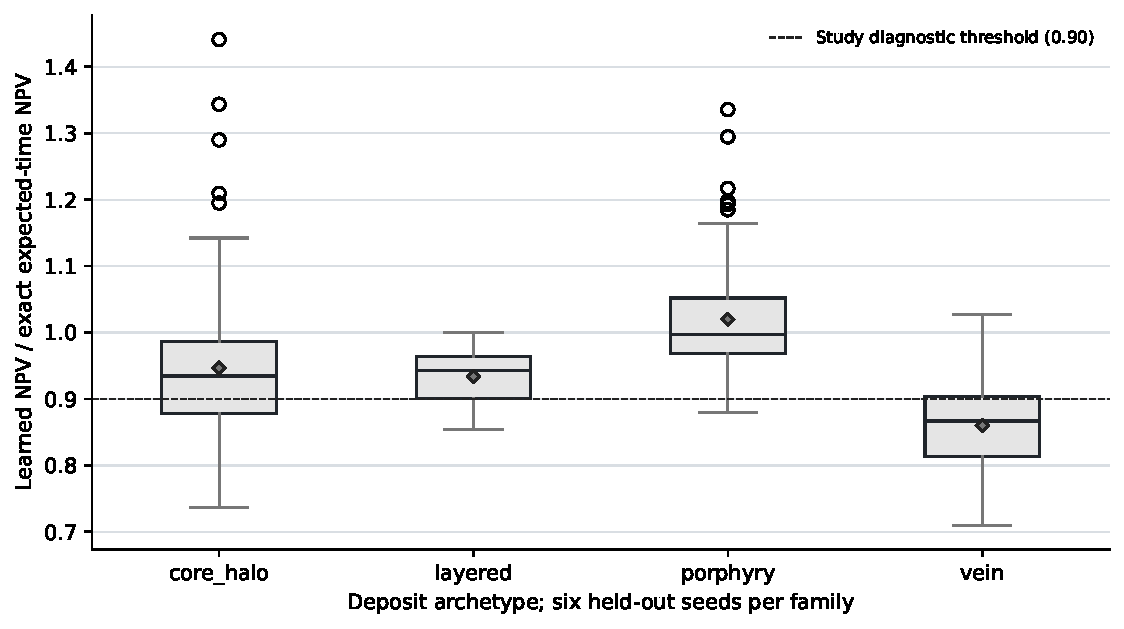
\includegraphics[width=0.86\textwidth]{figures/learned-holdout-by-archetype.pdf}\caption{Distribution of learned-to-exact expected-time schedule value over deposit-disjoint holdout cases, grouped by four generated archetypes and marked at the study threshold.}\label{fig:learned-holdout-by-archetype}\end{figure}
\begin{figure}[htbp]\centering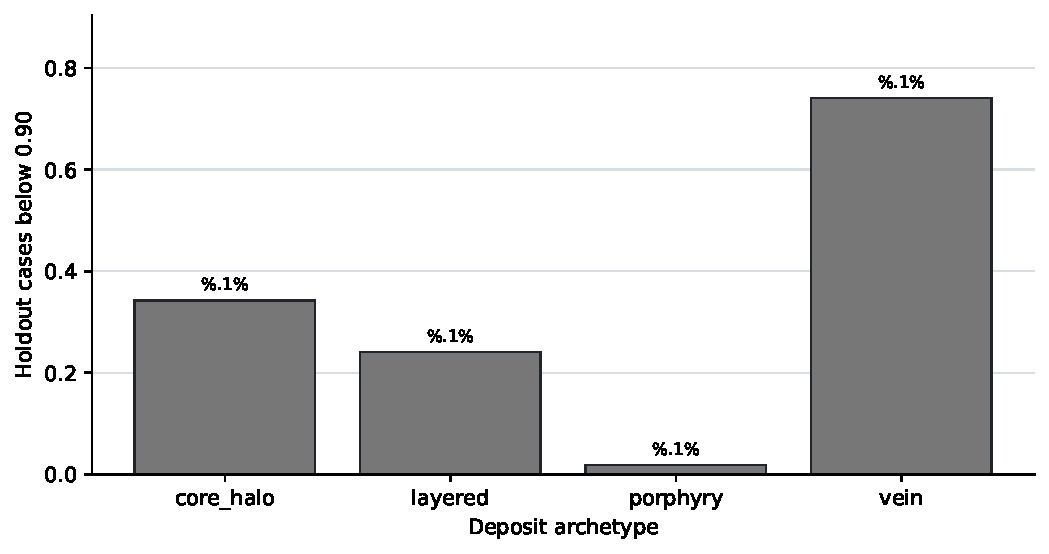
\includegraphics[width=0.82\textwidth]{figures/learned-failure-rate.pdf}\caption{Share of held-out generated cases below the fixed 0.90 value-ratio diagnostic, recomputed separately for each deposit archetype.}\label{fig:learned-failure-rate}\end{figure}
\clearpage

Figure~\ref{fig:learned-real-holdout} and Table~\ref{tab:real-holdout} retain the two benchmark cases separately: Newman1 is close to its exact expected-time comparator, while KD is below it. Two observations cannot estimate a cross-deposit transfer rate. The warning rule is also evaluated on a third disjoint set of 432 generated cases. Figure~\ref{fig:guard-confusion-matrix} shows 76 false negatives; Figure~\ref{fig:guard-thresholds} compares precision and recall with the frozen requirements, and Table~\ref{tab:guard-validation} includes the worst unflagged ratio. All three acceptance criteria fail. The warning rule therefore remains unavailable in the live lane; neither the figure nor the table supplies evidence for using it to screen real deposits.

\begin{figure}[htbp]\centering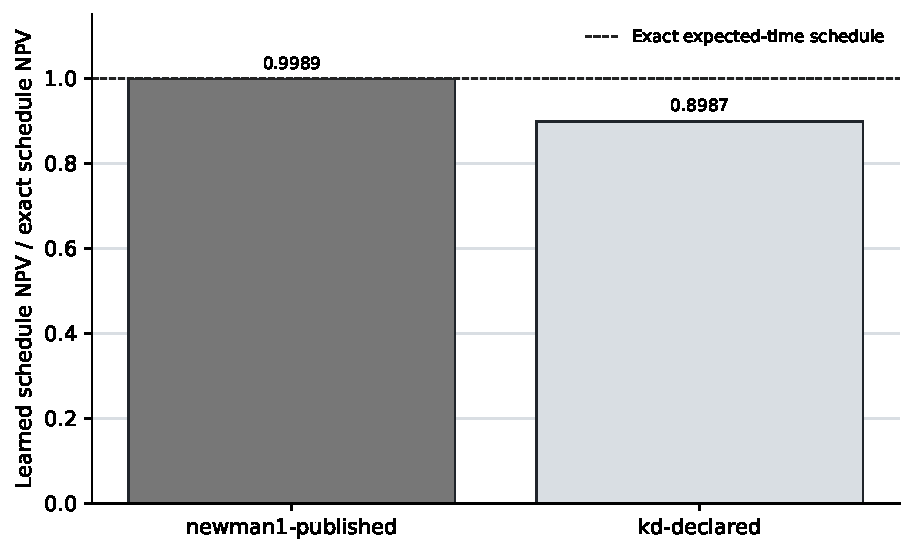
\includegraphics[width=0.7\textwidth]{figures/learned-real-holdout.pdf}\caption{Learned schedule value relative to exact expected-time ordering for the two scored MineLib cases, shown separately without pooling them into a transfer estimate.}\label{fig:learned-real-holdout}\end{figure}
\begin{figure}[htbp]\centering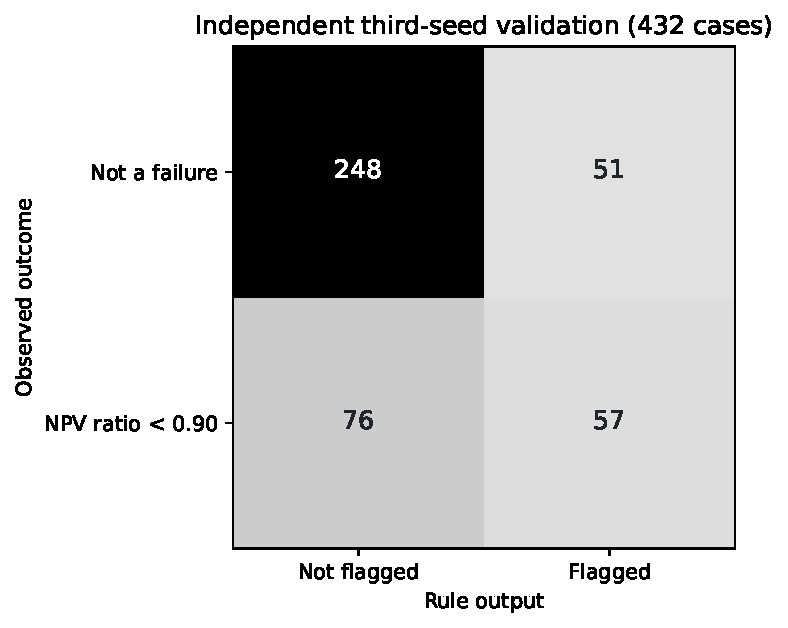
\includegraphics[width=0.66\textwidth]{figures/guard-confusion-matrix.pdf}\caption{Confusion matrix for the fixed archetype warning on its independent third-seed evaluation set, with missed low-value schedules visible explicitly.}\label{fig:guard-confusion-matrix}\end{figure}
\begin{figure}[htbp]\centering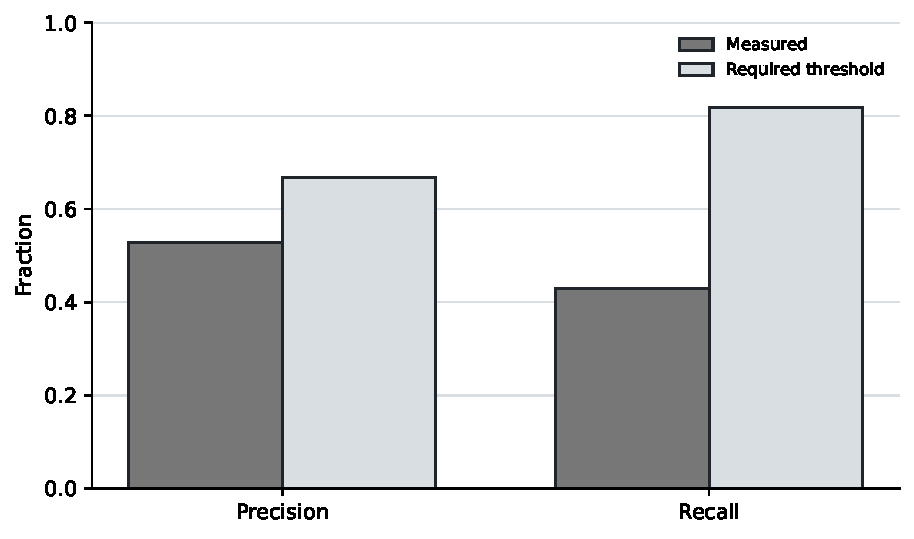
\includegraphics[width=0.72\textwidth]{figures/guard-thresholds.pdf}\caption{Measured guard precision and recall compared with the fixed acceptance thresholds defined before evaluation of the independent seed split.}\label{fig:guard-thresholds}\end{figure}

\begin{longtable}{lrrrrrr}
\caption{Deposit-disjoint synthetic evaluation results for the learned ordering and its exact comparator, grouped by archetype and measured on the same generated cases.}\label{tab:learned-by-archetype}\\
\toprule Archetype & $n$ & Median ratio & Mean ratio & 10th percentile & Minimum & Below 0.90 \\ \midrule
\endfirsthead\toprule Archetype & $n$ & Median ratio & Mean ratio & 10th percentile & Minimum & Below 0.90 \\ \midrule\endhead
core\_halo & 108 & 0.9348 & 0.9468 & 0.8482 & 0.7365 & 37/108 \\
layered & 108 & 0.9425 & 0.9337 & 0.8770 & 0.8536 & 26/108 \\
porphyry & 108 & 0.9972 & 1.0198 & 0.9484 & 0.8798 & 2/108 \\
vein & 108 & 0.8669 & 0.8600 & 0.7734 & 0.7101 & 80/108 \\
\bottomrule\end{longtable}

\begin{table}[htbp]\centering
\caption{The two licensed benchmark cases remain separate observations because they do not support an estimate of cross-deposit generalization.}\label{tab:real-holdout}
\begin{tabular}{lrrr}\toprule Case & Learned / exact ExTS & Spearman in pit & Scored \\ \midrule
newman1-published & 0.9989 & 0.2510 & yes \\
kd-declared & 0.8987 & 0.4214 & yes \\
\bottomrule\end{tabular}\end{table}

\begin{table}[htbp]\centering
\caption{The independently held-out warning rule is measured on 432 generated cases; the table preserves its false negatives and the thresholds it fails.}\label{tab:guard-validation}
\begin{tabular}{lrr}\toprule Measure & Measured & Required \\ \midrule
Precision & 0.5278 & $\geq 0.667$ \\
Recall & 0.4286 & $\geq 0.818$ \\
Worst unflagged ratio & 0.7322 & $\geq 0.7852$ \\
False negatives & 76 & 0 for complete detection \\
False positives & 51 & reported, not silently discounted \\
\bottomrule\end{tabular}\end{table}


\subsection{Reproducible system flow}
Figure~\ref{fig:system-architecture} maps the executable boundaries from case inputs through solving, independent evaluation, and the serialized replay products. The learned models are produced offline, while the deployed browser consumes static traces and uses its separate bounded interactive solver; the figure does not imply that the browser loads or trains the learned checkpoint. The source modules and contract schemas, rather than the diagram alone, define the exact data flow.

The first boundary is case admission: source dimensions, values, precedence, and capacities are converted into a versioned case description. The second boundary is method execution, which writes candidate schedules and solver outcomes without changing the source instance. The independent evaluator then recomputes feasibility and objective, and the contract layer serializes only the fields required for comparison and replay. The static site consumes the committed index and traces; it does not trigger a hidden full bake or update a published case when a reader changes a control. Synthetic interactive controls use a separately bounded calculation path and are visibly distinct from aggregate-only licensed benchmark records. These paths let readers distinguish a reproduced measurement, an interactive illustration, and a trained model artifact.

\begin{figure}[htbp]\centering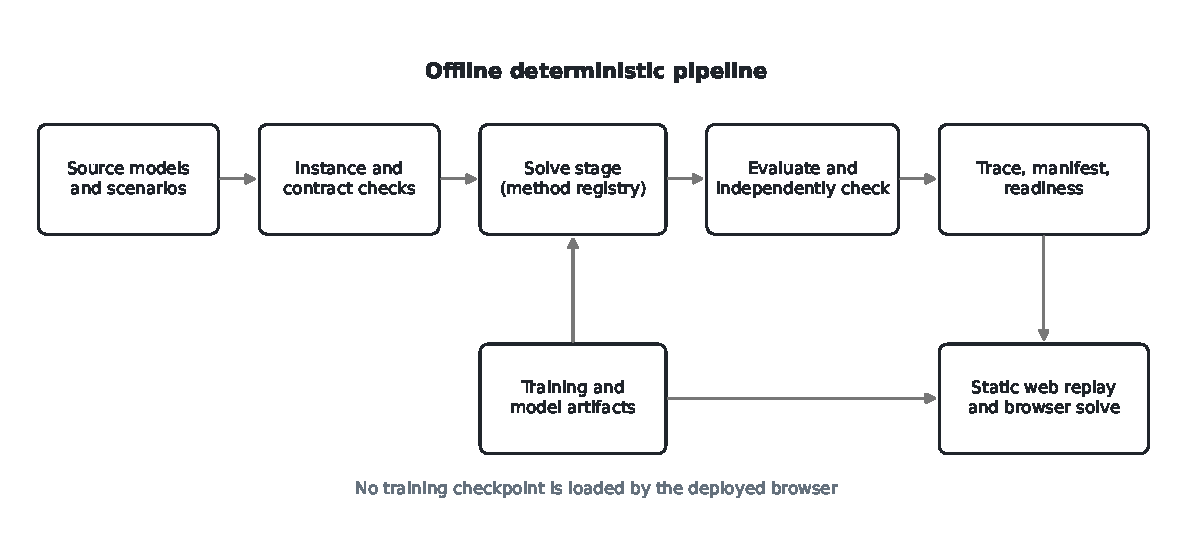
\includegraphics[width=\textwidth]{figures/system-architecture.pdf}\caption{PhaseFlow data path from model and scenario inputs through contract checks, registered solvers, independent evaluation, versioned traces, and browser replay.}\label{fig:system-architecture}\end{figure}
